\documentclass[12pt]{article}
\usepackage[top=1cm, bottom=3cm, right=2cm, left=2cm]{geometry}
\usepackage{amsfonts, amssymb, amsmath, hyperref}
\usepackage{graphicx}
\usepackage{wrapfig}
\usepackage{subcaption}
\usepackage[T1, T2A]{fontenc}% T2A for Cyrillic font encoding
\usepackage[english, russian]{babel}
\usepackage[justification=centering]{caption}
\usepackage[caption]

\pagestyle{empty}

\begin{document}
\title{\textbf{Лабораторная работа 2.2.6}\\[2pt]{Определение энергии активации по температурной зависимости вязкости жидкости}}
\date{\today}
\author{Татаурова Юлия Романовна}

\begin{document}
\maketitle
\textbf{Цель работы:} \\
1)Измерение скорости падения шариков при разной температуре жидкости;\\ 
2)Вычисление вязкости жидкости по закону Стокса и расчет энергии активации\\\indent

\textbf{Оборудование:} стеклянный цилиндр с исследуемой жидкостью; термостат;
секундомер; горизонтальный компаратор; мелкие шарики. 

\section*{Теоретические сведения}
\indent 
Для того, чтобы молекула жидкости перешла в новое состояние, она 
должна преодолеть участки с большой потенциальной энергией, 
превышающей среднюю тепловую энергию молекул. Т.е должна увеличиться 
на величину энергии активации $W$. Количество молекул с энергией, 
превышающей $W$ по формуле Больцмана:
\begin{equation}
    \eta \sim Ae^{\frac{W}{kT}}
\end{equation}
\indent
Чтобы исследовать температурную зависимость вязкости жидкости будем 
использовать метод Стокса. На тело, двигающееся в вязкой жидкости, 
действует сила сопротивления:
\begin{equation}
    F = 6\pi\eta r v
\end{equation}
\indent
Рассмотрим свободное падение шарика в вязкой жидкости (2ЗН):
\begin{equation}
    Vg(\rho - \rho_{\text{ж}}) - 6\pi\eta r v = V\rho \frac{dv}{dt} \label{eq:2newton}
\end{equation}
где $V$ - объем шарика, $\rho$ - его плотность, $\rho_{\text{ж}}$ - 
плотность жидкости. Тогда из \ref{eq:2newton} получаем:
\begin{align}
    v(t) &= v_{\text{уст}} - (v_{\text{уст}} - v_0) e^{-\frac{t}{\tau}}\\ 
    v_{\text{уст}} &= \frac{2}{9} g r^2 \frac{(\rho - \rho_{\text{ж}})}{\eta}\\ 
    \tau &= \frac{2}{9}\frac{r^2 \rho}{\eta}
\end{align}
где $v_0$ - начальная скорость шарика.\\
Тогда вязкость жидкости можно определить как:
\begin{equation}
    \eta = \frac{2}{9} g r^2 \frac{\rho - \rho_{\text{ж}}}{v_{\text{уст}}}
\end{equation}
% 17 and 23 april
Однако мы пользовались методикой Стокса, поэтому стоит так же проверить 
эту теорию. При выводе формулы Стокса предполагалось, что характер 
течения ламинарный, который можно описать числом Рейнольдса 
$Re = \frac{v r \rho_{\text{ж}}}{\eta} \approx 0.5$. \\ 
Также должно выполняться условие $t \gg \tau$

\section*{Экспериментальная установка}
\indent
Сосуд B с жидкостью помещен в рубашку D, засчет которой происходит нагрев 
жидкости. Cхема прибора изображена ниже. 
\begin{figure}[h!]
    \centering
    \begin{subfigure}{0.45\textwidth}
        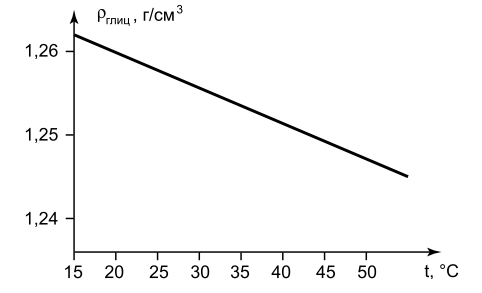
\includegraphics[height=5cm]{fluid2.png}
        \subcaption{Зависимость плотности глицерина от температуры}
    \end{subfigure}
\hfill
    \begin{subfigure}{0.45\textwidth}
        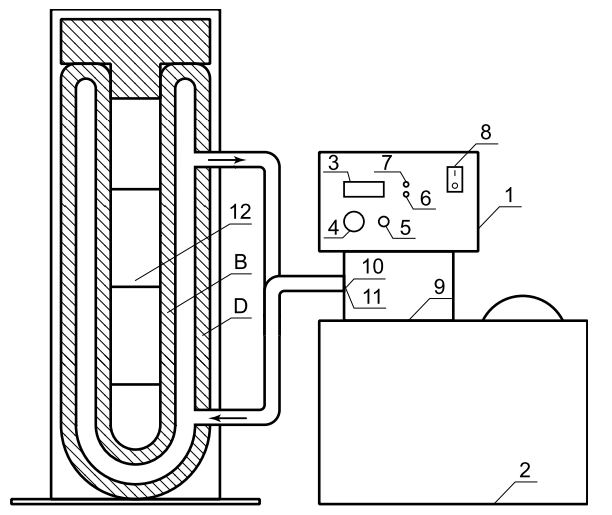
\includegraphics[height=5cm]{setup.png}
        \subcaption{Экспериментальная установка}
    \end{subfigure}
\end{figure}

\newpage

\section*{Экспериментальные данные}

\begin{table}[h!]
    \centering
    \caption{Зависимость скорости шариков от температуры}
    \begin{subtable}[h!]{0.49\textwidth}
        \begin{tabular}{|c|c|c|c|c|}
            \hline
            $d$, мм & 2.1 & 2 & 2 & 2.1\\\hline
            $\upsilon$, мм/c & 3.03 & 2.98 & 2.99 & 3.01\\\hline
        \end{tabular}
    \subcaption{Cкорость шариков при $T_1 = 21.6^{\circ}$C}
    \end{subtable}
    \hfill
    \begin{subtable}[h!]{0.49\textwidth}
        \begin{tabular}{|c|c|c|c|c|}
            \hline
            $d$, мм & 2.02 & 2.06 & 2.02 & 2\\\hline
            $\upsilon$, мм/c & 3.7 & 4.07 & 4.39 & 4.6\\\hline
        \end{tabular}
    \subcaption{Cкорость шариков при $T_2 = 30.4^{\circ}$C}
    \end{subtable}
    \vfill
    \begin{subtable}[h!]{0.49\textwidth}
        \begin{tabular}{|c|c|c|c|c|}
            \hline
            $d$, мм & 2.1 & 2 & 2.12 & 2.1\\\hline
            $\upsilon$, мм/c & \7.47 & 7.76 & 7.94 & 9.18\\\hline
        \end{tabular}
    \subcaption{Cкорость шариков при $T_3 = 40^{\circ}$C}
    \end{subtable}
    \hfill
    \begin{subtable}[h!]{0.49\textwidth}
        \begin{tabular}{|c|c|c|c|c|}
            \hline
            $d$, мм & 2.12 & 2 & 2.02 & 2\\\hline
            $\upsilon$, мм/c & 15.88 & 16.58 & 17.67 & 18.96\\\hline
        \end{tabular}
    \subcaption{Cкорость шариков при $T_4 = 50^{\circ}$C}
    \end{subtable}
\end{table}

\begin{figure*}[!h]
    \centering
    \begin{minipage}{0.42\textwidth}
        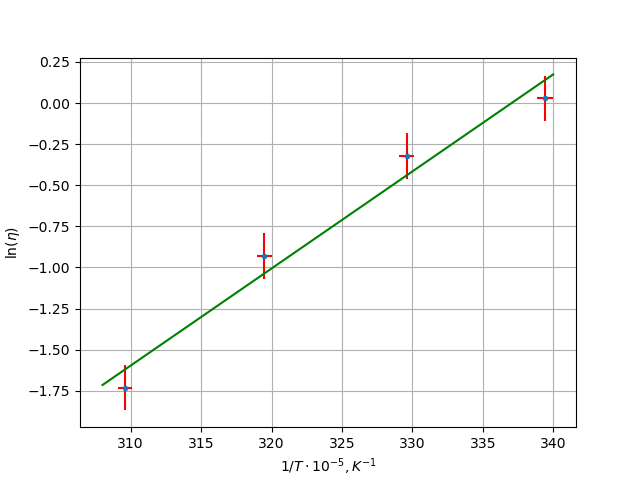
\includegraphics[height=8cm]{plot.png}
        \captionof{figure}{График зависимости $ln(\eta) (1/T)$}
    \end{minipage}
    \hfill
    \begin{minipage}{0.42\textwidth}
        \centering
        \begin{tabular}{|c|c|c|c|c|}
            \hline 
            $T^{\circ}C$ & 21.6& 30.4& 40& 50\\\hline
            $\eta$, Па$\cdot$c &1.028 & 0.723 & 0.395 & 0.177\\\hline
            $\tau$, c$\cdot 10^{-4}$ & 6 & 8 & 16 & 34\\\hline
            $Re \cdot 10^{-3}$ & 4 & 7 & 27 & 126\\\hline
            $S$, м$\cdot 10^{-7}$ & 18 & 35 & 130 & 590\\\hline
            $\rho_{\text{жид}}$, г/см$^3$ & 1256 & 1254 & 1251 & 1248\\\hline
        \end{tabular}
        \captionof{table}{Результаты вычислений}
    \end{minipage}
\end{figure*}
Из гарфика $\frac{W}{k} = 5901 \rightarrow W \approx 0.5$ эВ.\\

\subsection*{Результаты и выводы}
$$\sigma_{\text{t}} = \sqrt{\sigma_{\text{приб}}^2 + \frac{\sum_{i=1}^{n} (t_{\text{i}} - t_{\text{ср}})^2}{(n-1)n}} = 0.69\text{ с ; }
    \varepsilon_{\upsilon} = \sqrt{\left (\frac{\sigma_{\text{t}}}{t_{\text{min}}}\right )^2 + \left (\frac{\Delta l}{l}\right )^2} = 13.3 \%  $$
\\
В ходе эксперимента были вычислены значения коэффициента вязкости 
глицерина при зарных температурах. Так же можно заметить, что течение в эксперименте 
можно считать ламинарным, т.к число Рейнольдса оказалось достаточно маленьким ($\sim 10^{-2}$). 
Помимо этого во всех экспериментах время релаксации, как и путь релаксации намного 
меньше измеряемых величин, поэтому движение шарика во время измерений можно 
действительно считать установившимся. 




\end{document}
